\begin{figure}[h]
    \centering
    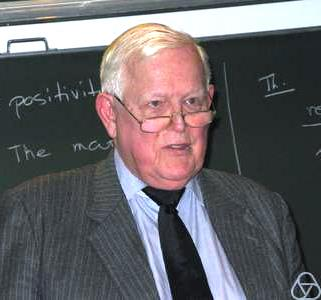
\includegraphics[scale=0.8]{AerospaceApplications/images/Kalman.jpg}
    \caption{Rudolf Kalman (1930-2016)}  
\end{figure}
\noindent
In many real-world applications not all the state variables are measurable: sometimes either sensors may be expensive or there is no available space. In other situations could be useful having more than one sensor for the same state variable for redundancy, even though a variable is measured relevant \textbf{disturbances} and \textbf{noises} could appear.\\

In all these situations \textbf{Observers and Filters} are employed, they are devices which implement some \textbf{algorithms} in order to estimate the state variables from the measurement of input to the system, and the output from the system. The difference between Observer and Filter is that in the first case no assumptions are available on the disturbance/noise characteristics, in the latter case we call \textit{filter} a device which takes into account also the presence of measurement noise and/or the presence of disturbances. This aspect in real-world situations ought to be taken into account. Widely used observers are:
\vspace{-0.2cm }
\begin{enumerate}
    \itemsep-0.2cm
    \item \textbf{Linear Kalman Filter}; 
    \item \textbf{Extended Kalman Filter}.
\end{enumerate}
[They were introduced by Kalman starting from the following scientific paper: \textsf{Kalman, R.E., A new approach to linear filtering and prediction problems, in Journal of Basic Engineering, vol. 82, n. 1, 1960}].

\section{Linear Kalman Filter}
This has been developed even in the continuous time (CT) that in the discrete time (DT). The \textbf{Kalman Filter} description in discrete time is simpler and more suitable for \textit{on-line implementation} where sampled data (in discrete time) are used. Moreover the discrete time description is useful for the implementation of such method on microprocessors. For this aim consider a \textbf{Discrete time Linear Time Varying (LTV)} system described by the equations:
\begin{equation}
    \begin{aligned}
        &x_{k+1} = F_k x_k + G_k u_k + d_k\\
        &y_k = H_k x_k + d_k^y
    \end{aligned}
\end{equation}
wher $k\in\mathbb{Z}$ is the time index, while $d_k$ and $d_k^y$ are respectively the \textbf{process disturbance} and \textbf{measurement noise}. The state $x_k$ and the disturbances are not known, while the input  $u_k$ and the output $y_k$ are measured.\\
{\large{
    \color{red}
    \begin{quotation}
        The \textbf{objective} of Kalman's algorithm is to estimate possibly in an accurate way the state $\hat{x}_k$ of $x_k$ from the \textbf{current} and \textbf{past} measurements of the input and the output. 
    \end{quotation}
}}

Like also other observer algorithms, the Kalman filter is based on the following two operations:
\begin{enumerate}
    \item \textsf{\textbf{Prediction}}. At time $k-1$ a \textbf{prediction} $x_k^p$ is computed by using the \textbf{system model} 
    \begin{equation}
        x_k^p  = F_{k-1}\hat{x}_{k-1} + G_{k-1} u_{k-1}
    \end{equation}
    \item \textsf{\textbf{Update of the estimate}}. At time $k$, the prediction previously done is \textit{corrected} using the output $y_k$ in order to give a \textit{more accurate} estimate of the state. Technically speaking:
    \begin{equation}
        \begin{aligned}
            &\hat{x}_k = x_k^p + K_k \delta y_k\\
            &\delta y_k = y_k - y_k^p = y_k - H_k y_k^p
        \end{aligned}
    \end{equation} 
    where $K_k$ is chosen in order to minimize the \textbf{variance} of the \textit{estimation error norm} $\mathbb{E}\big[
        \Vert x_k-\hat{x}_k \Vert_2^2
    \big]$ when the variance of the estimation error the error itself becomes small, $y_k^p$ is the \textbf{predicted output}, i.e. the output computed using the system model ($H_k$) and the \textbf{predicted state} $x_k$.
\end{enumerate}
In order to introduce the algorithm is useful giving some definitions: 
\begin{itemize}
    \itemsep0em
    \item $x_k^p$: prediction of $x_k$ at time $k-1$
    \item $\hat{x}_k$ is the \textbf{estimate} of $x_k$ at time $\delta x_k=x_k-x_k^p$ is the \textit{state prediction error}
    \item $\tilde{x}_k\doteq x_k-\hat{x}_k$  is the \textit{state estimation error}
    \item $P_k^p\doteq\mathbb{E}[\delta x_k \delta x_k^\textsf{T}]$ is the \textit{covariance matrix of the prediction error}
    \item $P_k\doteq \mathbb{E}[\tilde{x}_k \tilde{x}_k^{\textsf{T}}]$ is thr \textit{covariance matrix of the estimation error}
    \item $Q_d \doteq \mathbb{E}[d_k d_k^T]$ is the \textit{covariance matrix of $d_k$}
    \item $R_d \doteq \mathbb{E}[d_k^y {d_k^y}^{\textsf{T}}]$ is the \textit{covariance matrix of $d_k^y$}
\end{itemize}

\noindent
Before starting with the algorithm some \textbf{preliminary operations} have to be done:
\begin{enumerate}
    \itemsep-0.2em
    \item \textsf{\textbf{Design of $\mathsf{R_d}$ and $\mathsf{Q_d}$}} typically based on the probabilistic available information on the noise/disturbance, commonly the are chosen to be diagonal with the variance of $d_k$ and $d_k^y$ on the diagonal. Most of the times they require tuning because not always one have precise information on the noise structure;
    \item \textsf{ \textbf{Initialization}} by setting:
    \begin{itemize}
        \itemsep0em
        \item $\hat{x}_0=0$, the initial estimated state; 
        \item $P_0$ the initial covariance matrix of the estimation error (tipically assumed to be the identity $I$).
    \end{itemize}
\end{enumerate}
After the discussion on these important details, we are ready to present the \textsf{Kalman Algorithm}:\\

\hspace*{-5mm}
\begin{tikzpicture}
\node [mybox] (box){%
    \begin{minipage}{.96\textwidth}     
    \normalsize{
        \textsf{\textbf{Kalman Filter algorithm}}
        \begin{enumerate}
            \itemsep-0.2em
            \item \textsf{Prediction}:
            \begin{align*}
                &x_k^p = F_{k-1} \hat{x}_{k-1} + G_{k-1} u_{k-1}\\
                &P_k^p = F_{k-1}P_{k-1}F_{k-1}^{\textsf{T}}+Q_d
            \end{align*}
            \item \textsf{Update}:
            \begin{align*}
                &S_k = H_k P_k^p H_k^{\textsf{T}} + R_d\\
                &K_k = P_k^p H_k^{\textsf{T}} S_k^{-1}\\
                &\delta y_k = y_k - H_k x_k^p\\
                &\hat{x}_k = x_k^p + K_k \delta y_k\\
                &P_k = (I-K_k H_k)P_k^p
            \end{align*}
        \end{enumerate}
    }
    
    \end{minipage}
};
\end{tikzpicture}%

The presented algorithm uses some assumptions on the stochastic part of the problem that is related to the noise/disturbance. In particular, without entry too much into details, the noises are assumed to be iid (independent and identically distributed), \textit{cross-uncorrelation} of noise and input-noise is required. Finally an important requisite which is always needed when an observer has to be employed is the \textbf{global observability}. \\
There is the important following theorem of which the proof is omitted, that state:\\

\hspace*{-5mm}
\begin{tikzpicture}
\node [mybox] (box){%
    \begin{minipage}{.96\textwidth}     %Larghezza del box
    \large{
        \textsf{\textbf{Theorem}}\\
        The linear Kalman Filter built as presented guarantees an estimation error with \textbf{zero mean} and \textbf{minimum variance}:
        \begin{equation*}
            K_k = \text{arg}\min_{\mathcal{K}} \mathbb{E} \big[
                \Vert x_k-\hat{x}_k \Vert_2^2
            \big]
        \end{equation*}
    }
    \end{minipage}
};
\end{tikzpicture}%

\subsection{Linear Time Invariant case (LTI)}
Let us consider now the case in which the matrices $F, G, H$ are linear time invariant (LTI), that is they do not depend on the time $k$. The system becomes:
\begin{equation}
    \begin{aligned}
        &x_{k+1} = Fx_k + Gu_k + d_k\\
        &y_k = H x_k + d_k^y
    \end{aligned}
\end{equation}
where the quantities $d_k$, $d_k^y$ are the noises. 

It can be proven that if the covariance matrices $Q_d, R_d$ of the process noise and measurement noise respectively are \textbf{definite positive}, that is $Q_d, R_d \succ 0$ and $(F, H)$ is observable, then
\begin{equation*}
    \lim_{k\to\infty} P_k^p \to \bar{P}
\end{equation*}
This implies that also $P_k$, $S_k$, $K_k$ converges to constant values $P, S, K$ as $k\to\infty$. Using these information we can derive the asymptotic equations for the following matrices:
\begin{align*}
    &\bar{P} = FPF^{\textsf{T}} + Q_d \\
    &S = H\bar{P}H^{\textsf{T}}+ R_d \\
    &K = \bar{P}H^{\textsf{T}}S^{-1}\\
    &P = (I-KH) \bar{P}
\end{align*}
By eliminating P and S we can write the following two equations: 
\begin{align}
    &\bar{P}  F(\bar{P} - \bar{P}H^{\textsf{T}} (H\bar{P}H^{\textsf{T}}+R_d)^{-1} H \bar{P})F^{\textsf{T}} + Q_d\\
    &K = \bar{P}H^{\textsf{T}}(H\bar{P}H^{\textsf{T}}+R_d)^{-1}
\end{align}
The first of these two equations is called \textit{discrete algebraic Riccati equation}, the second is the filter gain matrix. Then we have the predicted and estimated state equations:
\begin{align*}
    &x_k^p = F \hat{x}_{k-1} + G u_{k-1}\\
    &\hat{x}_k = x_k^p + K (y_k-H x_k^p)
\end{align*}
We have to replace the definition of $x_{k-1}$ in the first equation, in this way we will obtain: 
\begin{align*}
    x_k^p &= F [x_{k-1}^p + K (y_{k-1} - H x_{k-1}^p)] + G u_{k-1} =\\
    & F[x_{k-1}^p + K y_{k-1} -KH x_{k-1}^p] + G u_{k-1}=\\
    & F x_{k-1}^p + FK y_{k-1} - FKH x_{k-1}^p + G u_{k-1}
    \overset{L \doteq FK }{=}\\
    & (F-LH) x_{k-1}^p + L y_{k-1} + G u_{k-1}
\end{align*}
The equations describing the \textit{prediction} and the \textit{estimation} of the state, at the end of the day are:
\begin{align}
    &x_k^p = (F-LH) x_{k-1}^p + L y_{k-1} + G u_{k-1}\\
    &\hat{x}_k = x_k^p + K (y_k-H x_k^p)
\end{align}
\noindent 
The LTI case is a subcase of LTV, the properties on the error are required also here, the matrix $K$ previously defined ensures the minimum variance of the estimation error. The \texttt{Matlab} function \texttt{kalman} gives $L$ and $K$.
 
\section{Extended Kalman Filter (EKF)}
Here we want to define an algorithm for the estimation for the nonlinear case. For this purpose we define the following \textit{discrete-time nonlinear system}:
\begin{align*}
    &x_{k+1} = f(x_k, u_k) + d_k\\
    &y_k = h(x_k) + d_k^y
\end{align*} 

The matrices $F_k$ and $H_k$ are obtained by linearizing the nonlinear functions $f$ and $h$ along the estimated trajectory. In particular:
\begin{itemize}
    \item $F_k \doteq \frac{\partial f}{\partial x} (\hat{x}_k, u_k)$: which is substancially the Jacobian of $f$ computed at $(\hat{x}_k, u_k)$
    \item $H_k \doteq \frac{\partial h}{\partial x}(\hat{x}_k)$: which is the Jacobian of $h$ computed at $\hat{x}_k$
\end{itemize}
Notation, Definitions, design of $Q_d$ and $R_d$ and initialization are the same than in the linear case, also the algorithm has not big differences.\\

\hspace*{-5mm}
\begin{tikzpicture}
\node [mybox] (box){%
    \begin{minipage}{.96\textwidth}     
    \normalsize{
        \textsf{\textbf{Extended Kalman Filter algorithm}}
        \begin{enumerate}
            \itemsep-0.2em
            \item \textsf{Prediction}:
            \begin{align*}
                &x_k^p =  f(\hat{x}_{k-1}, u_{k-1})\\
                &P_k^p = F_{k-1}P_{k-1}F_{k-1}^{\textsf{T}}+Q_d
            \end{align*}
            \item \textsf{Update}:
            \begin{align*}
                &S_k = H_k P_k^p H_k^{\textsf{T}} + R_d\\
                &K_k = P_k^p H_k^{\textsf{T}} S_k^{-1}\\
                &\delta y_k = y_k -  h(x_k^p)\\
                &\hat{x}_k = x_k^p + K_k \delta y_k\\
                &P_k = (I-K_k H_k)P_k^p
            \end{align*}
        \end{enumerate}
    }
    \end{minipage}
};
\end{tikzpicture}%

There are some \textbf{advantages} in using an EKF. At first the algorithm in a relatively simple way provides a way to estimate the state variables for a nonlinear system and it works well in many real-world applications. There are also \textbf{drawbacks} for instance EKF is not optimal, due to the fact some approximation are used the stability is NOT guaranteed, at the end it is remarkable that there is \textit{high sensibility to the initial conditions}.

\subsection{Discussion}
\subsubsection{Prediction and correction}
We have seen in EK and EKF algorithms that two steps are required: (i) the \textbf{prediction} is made by using the model of the system in a preliminar way; (ii) It is then important to \textbf{CORRECTS} the prediction by using the measurement of the output $y_k$, which is very important because increases the accuracy of the overall filter stability providing the possibility to \textbf{filter} measurement noise.

\subsubsection{Current/Delayed versions }
This is a more technical detail which reguards the implementation of the filter in embedded systems. In particular there are two possible approach: 
\begin{itemize}
    \item \textsf{Current version}. It uses all the measurement up to time $k$, the prediction equation is used $$\hat{x}_k = x_k^p + K_k \delta y_k$$ 
    \item \textsf{Delayed version}. It uses all the measurements (samples) up to time $k-1$, for this reason the estimation equation is used $$x_k^p =  f(\hat{x}_{k-1}, u_{k-1})$$
\end{itemize}
The latter is easier to implement because often it is not possible to measure and compute the state at the same time.

\section{Application: Spacecraft attitude determination}
In the \textit{aerospace field} Kalman filters are very used as a \textbf{virtual sensor}, in many situation there is no possibility to use the sensors because they are expensive or simply there is no space to install them. Then, the \textbf{estimation} acts a crucial role for the exposed reason. One of the application in aerospace field is the \textbf{attitude determination}. \\
Here the state equations are in the following form: 
\begin{align*}
    &\mathbf{\dot{x}} = \mathbf{A(x)x+Bu+Bd}^u\\
    &y=h(\mathbf{x})+\mathbf{d}^y
\end{align*}

\begin{equation*}
    \textbf{x} \doteq \begin{bmatrix}
        \ \mathfrak{q} \ \\
        \ \boldsymbol{\omega} \ 
    \end{bmatrix}, \quad 
    \mathbf{A(x)} \doteq \begin{bmatrix}
        0& \frac{1}{2}\mathbf{Q }\\
        0& -\mathbf{J}^{-1}\boldsymbol{\omega}\times \mathbf{J}
    \end{bmatrix}, \quad 
    \mathbf{B} \doteq \begin{bmatrix}
        0 \\ \mathbf{J}^{-1}
    \end{bmatrix}.
\end{equation*}

This is a \textbf{continuous time} system, we use the \textbf{forward Euler method} in order to discretize it by obtaining:
\begin{align*}
    &\mathbf{x}_{k+1} = \mathbf{F(x_k)x_k+G u_k + d_k}\\
    &\mathbf{y}_k = h(\mathbf{x_k})+\mathbf{d}_k^y
\end{align*}
Where $\mathbf{F(\hat{x}_k)} \doteq \mathbf{I}+\tau \mathbf{A(x_k)}$, $\mathbf{G}\doteq\tau\mathbf{B}$ and $\mathbf{d}_k = \tau \mathbf{Bd}_k^u$ and $\tau$ is the \textit{sampling time}. 
The equations are \textbf{quasi-LTV}: the matrix $\mathbf{F(\hat{x}_k)}$ depends on the state. In the standard LTV system the matrix $\mathbf{F_k}$ is known and it is independent on the state. Here $\mathbf{F}$ is not exactly known and depends on the state. At the end of the day the EKF matrices can be taken like this: 
\begin{align*}
    &\mathbf{F}_k \doteq F(\hat{x}_k) \quad \text{or} \quad
     \mathbf{F}_k \doteq \frac{\partial f}{\partial \mathbf{x}}(\hat{x}_k, \mathbf{u}_k)\\
    &\mathbf{H}_k \doteq \frac{\partial h}{\partial \mathbf{x}}(\hat{\mathbf{x}}_k)
\end{align*}

\noindent
In general the two $\mathbf{F}$ matrices are similar but not equal.\\

\hspace*{-5mm}
\begin{tikzpicture}
\node [mybox] (box){%
    \begin{minipage}{.96\textwidth}     
    \normalsize{
        \textsf{\textbf{EKF algorithm (for attitude determination)}}
        \begin{enumerate}
            \itemsep-0.2em
            \item \textsf{Prediction}:
            \begin{align*}
                &x_k^p =  \mathbf{F_{k-1}} \hat{\mathbf{x}}_{k-1} + \mathbf{G} u_{k-1}\\
                &\mathbf{P}_k^p = \mathbf{F}_{k-1}\mathbf{P}_{k-1}\mathbf{F}_{k-1}^{\textsf{T}}+\mathbf{Q}_d
            \end{align*}
            \item \textsf{Update}:
            \begin{align*}
                &\mathbf{S}_k = \mathbf{H}_k \mathbf{P}_k^p \mathbf{H}_k^{\textsf{T}} + \mathbf{R}_d\\
                &\mathbf{K}_k = \mathbf{P}_k^p \mathbf{H}_k^{\textsf{T}} \mathbf{S}_k^{-1}\\
                &\delta \mathbf{y}_k = \mathbf{y}_k -  h(x_k^p)\\
                &\hat{\mathbf{x}}_k = \mathbf{x}_k^p + \mathbf{K}_k \delta \mathbf{y}_k\\
                &P_k = (\mathbf{I}-\mathbf{K}_k \mathbf{H}_k)\mathbf{P}_k^p
            \end{align*}
        \end{enumerate}
    }
    \end{minipage}
};
\end{tikzpicture}%




